\chapter*{Практика 7. Эквалайзирование и OFDM демодуляция}
\addcontentsline{toc}{chapter}{Практика 7. Эквалайзирование и OFDM демодуляция}
\label{ch:7_practice}

\textit{\textbf{Задание:}} Реализовать приёмную часть системы связи.

\begin{itemize}
    \item Разработан OFDM демодулятор:
    \begin{itemize}
        \item Удаление циклического префикса
        \item БПФ
        \item Оценка канала по пилотным символам
        \item Эквалайзирование
        \item Удаление нулевых поднесущих
    \end{itemize}
    \item Реализовано восстановление исходных данных
\end{itemize}

\begin{figure}[ht]
    \centering
    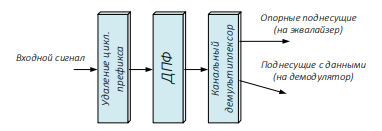
\includegraphics[width=0.8\textwidth]{ofdm_demodulator.png}
    \caption{Структура OFDM демодулятора и эквалайзера}
    \label{fig:ofdm_demodulator}
\end{figure}

\begin{figure}[ht]
    \centering
    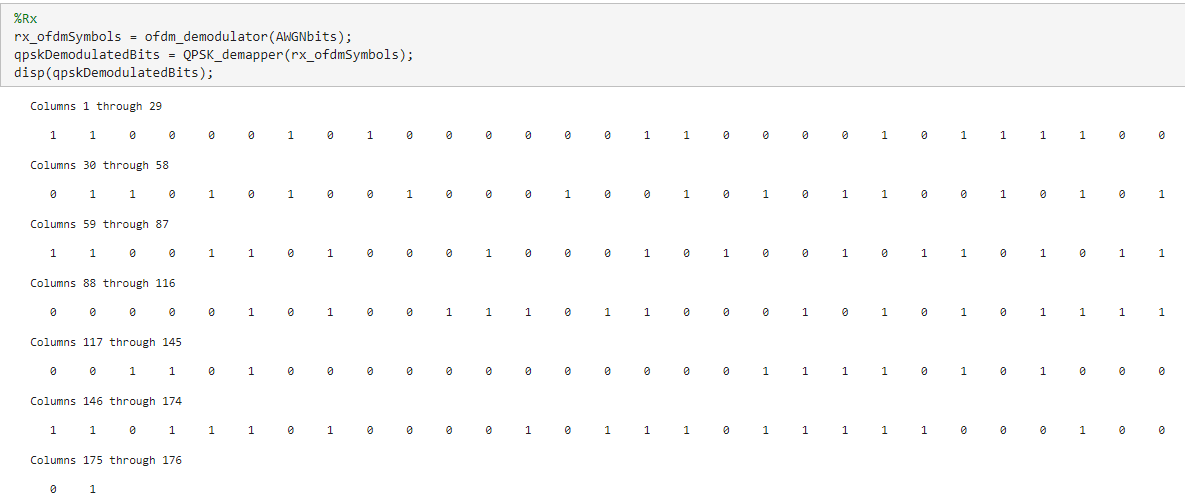
\includegraphics[width=0.8\textwidth]{7practice_result.png}
    \caption{Результат седьмой практики}
    \label{fig:7practice_result}
\end{figure}
